\begin{table}[htbp]
	\centering
	\scriptsize
	\subtable[Triple Naive]{%
		\begin{tabular}{l | ccccc} % creating eight columns
	 \hline
		\hline
		Triple  & \multicolumn{5}{c}{Slots}  \\
		in & \multicolumn{5}{c}{Number}  \\
		Window  & 1 & 10 & 100 & 1000&10000\\
		\hline
		1	   & \begin{minipage}{.15\textwidth}\vspace{2pt}     							
     			 	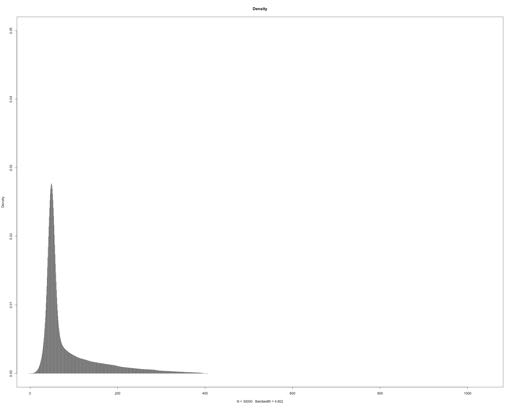
\includegraphics[width=\linewidth]{images/mema-dens-triple/N1}
    				 \end{minipage}\\			
		10	   & \begin{minipage}{.15\textwidth}\vspace{2pt}     							
     			 	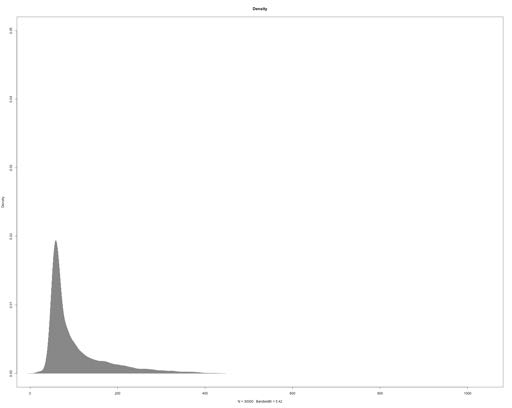
\includegraphics[width=\linewidth]{images/mema-dens-triple/N2}
    				\end{minipage}
    			   & \begin{minipage}{.15\textwidth}\vspace{2pt}     							
     			 	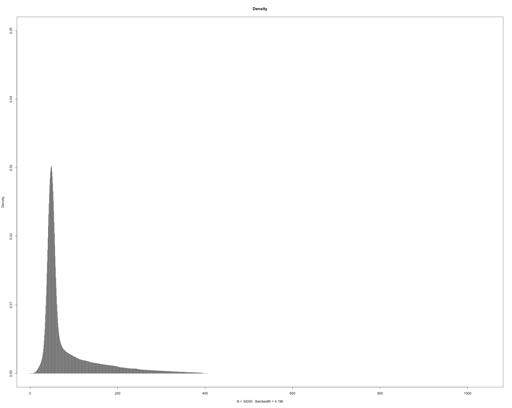
\includegraphics[width=\linewidth]{images/mema-dens-triple/N6}
    				 \end{minipage}\\		
		100	   & \begin{minipage}{.15\textwidth}\vspace{2pt}     							
     			 	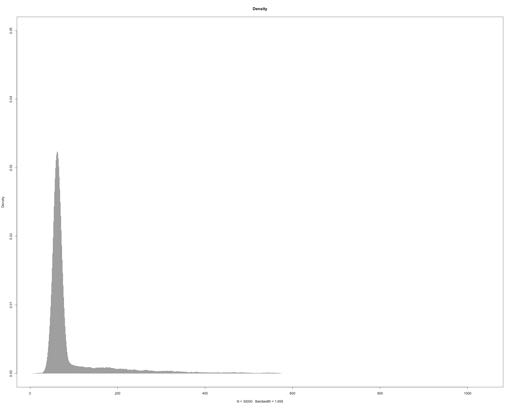
\includegraphics[width=\linewidth]{images/mema-dens-triple/N3}
    				 \end{minipage}
    			   & \begin{minipage}{.15\textwidth}\vspace{2pt}     							
     			 	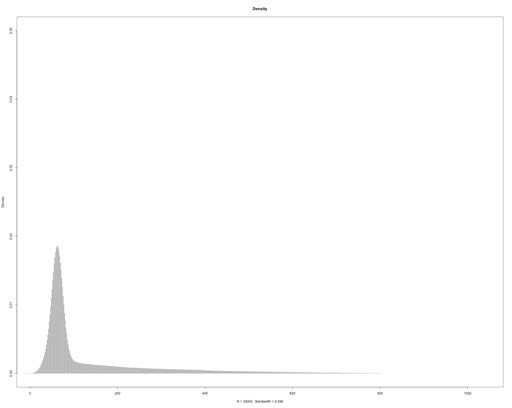
\includegraphics[width=\linewidth]{images/mema-dens-triple/N7}
    				 \end{minipage}
    			   &	 \begin{minipage}{.15\textwidth}\vspace{2pt}     							
     			 	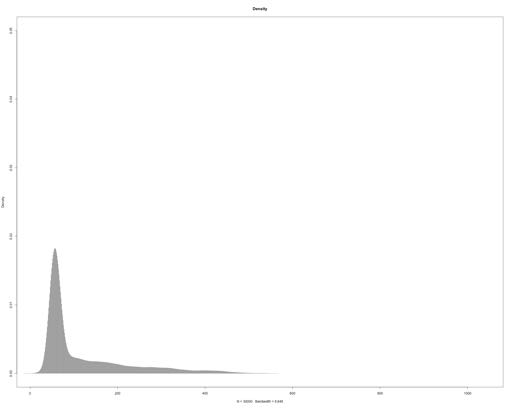
\includegraphics[width=\linewidth]{images/mema-dens-triple/N10}
    				 \end{minipage}\\	
		1000   &	 \begin{minipage}{.15\textwidth}\vspace{2pt}     							
     			 	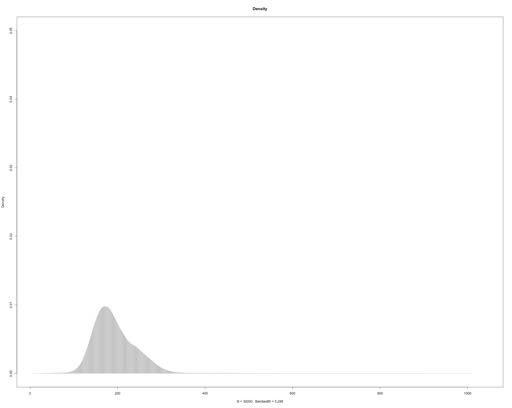
\includegraphics[width=\linewidth]{images/mema-dens-triple/N4}
    				 \end{minipage}
    			   &	 \begin{minipage}{.15\textwidth}\vspace{2pt}     							
     			 	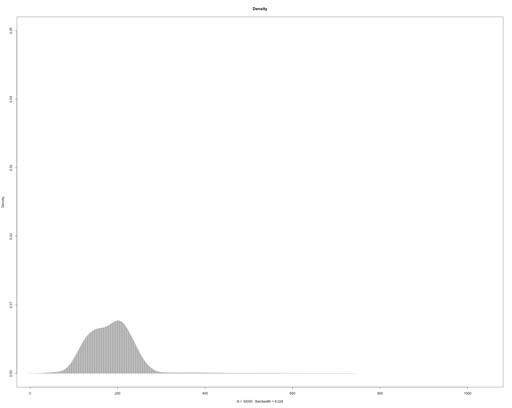
\includegraphics[width=\linewidth]{images/mema-dens-triple/N8}
    				 \end{minipage}
    			   &	 \begin{minipage}{.15\textwidth}\vspace{2pt}     							
     			 	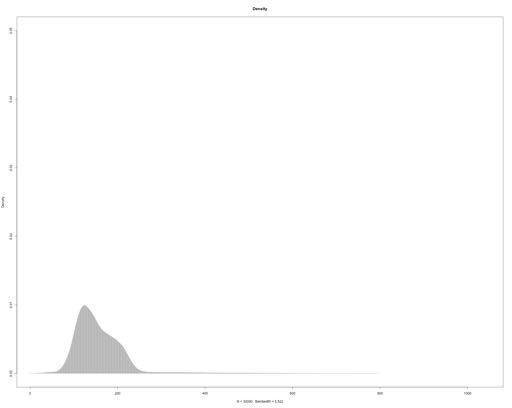
\includegraphics[width=\linewidth]{images/mema-dens-triple/N11}
    				 \end{minipage}
    			   &	 \begin{minipage}{.15\textwidth}\vspace{2pt}     							
     			 	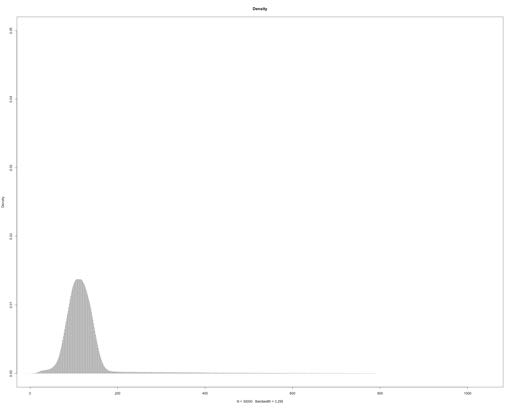
\includegraphics[width=\linewidth]{images/mema-dens-triple/N13}
    				 \end{minipage}\\
		10000  &	 \begin{minipage}{.15\textwidth}\vspace{2pt}     							
     			 	
\includegraphics[width=\linewidth]{images/mema-dens-triple/N5}
    				 \end{minipage}
    			   &	 \begin{minipage}{.15\textwidth}\vspace{2pt}     							
     			 	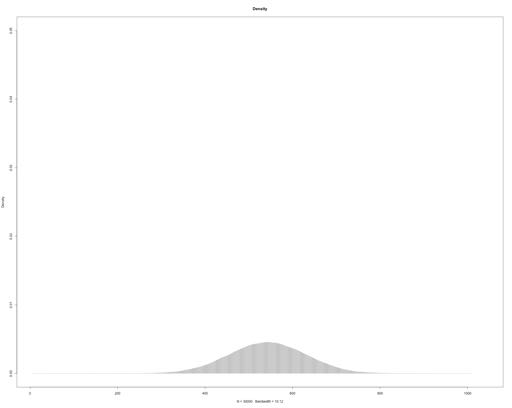
\includegraphics[width=\linewidth]{images/mema-dens-triple/N9}
    				 \end{minipage}
    			   &	 \begin{minipage}{.15\textwidth}\vspace{2pt}     							
     			 	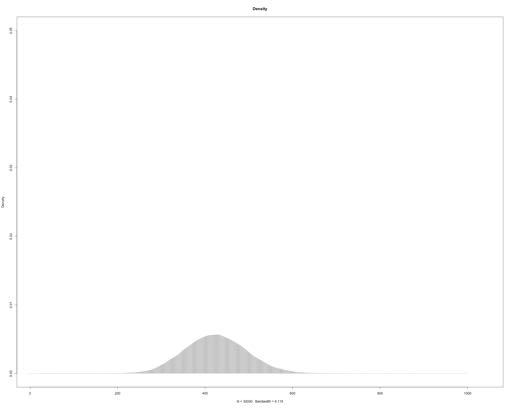
\includegraphics[width=\linewidth]{images/mema-dens-triple/N12}
    				 \end{minipage}
    			   &	 \begin{minipage}{.15\textwidth}\vspace{2pt}     							
     			 	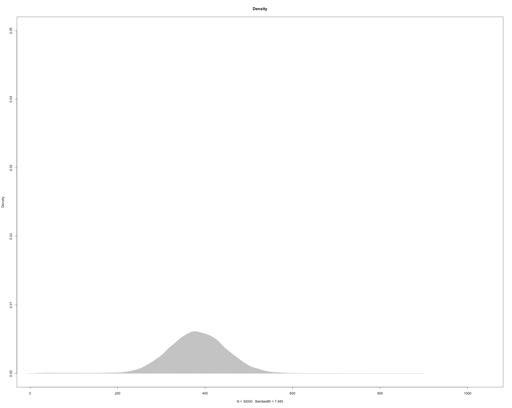
\includegraphics[width=\linewidth]{images/mema-dens-triple/N14}
    				 \end{minipage}
    			   &	 \begin{minipage}{.15\textwidth}\vspace{2pt}     							
     			 	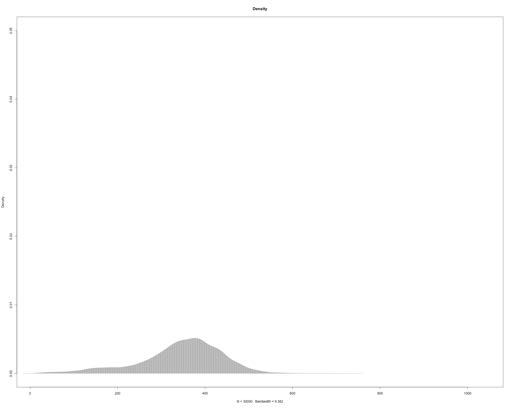
\includegraphics[width=\linewidth]{images/mema-dens-triple/N15}
    				 \end{minipage}\\
		\hline % inserts single-line
	 \end{tabular}
	}
	\subtable[Triple Incremental]{%
		\begin{tabular}{l | ccccc} % creating eight columns
	  	\hline
					\hline
		Triple  & \multicolumn{5}{c}{Slots}  \\
		in & \multicolumn{5}{c}{Number}  \\
		Window  & 1 & 10 & 100 & 1000&10000\\
		\hline
		1	   &\begin{minipage}{.15\textwidth}\vspace{2pt}     							
     			 	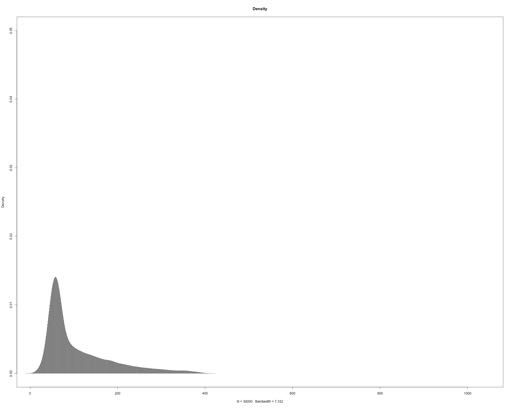
\includegraphics[width=\linewidth]{images/mema-dens-triple/I1}
    				 \end{minipage}\\			
		10	   & \begin{minipage}{.15\textwidth}\vspace{2pt}     							
     			 	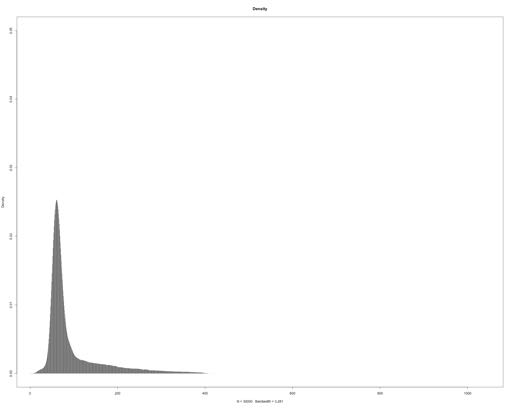
\includegraphics[width=\linewidth]{images/mema-dens-triple/I2}
    				\end{minipage}
    			   & \begin{minipage}{.15\textwidth}\vspace{2pt}     							
     			 	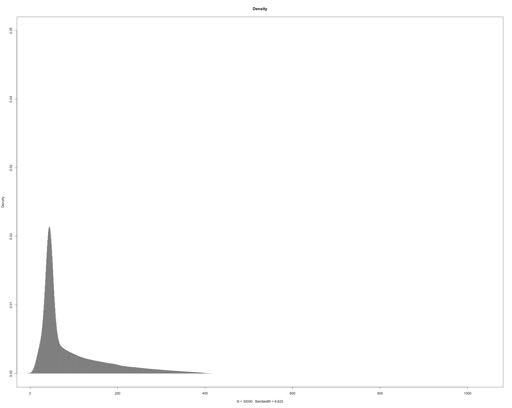
\includegraphics[width=\linewidth]{images/mema-dens-triple/I6}
    				 \end{minipage}\\		
		100	   & \begin{minipage}{.15\textwidth}\vspace{2pt}     							
     			 	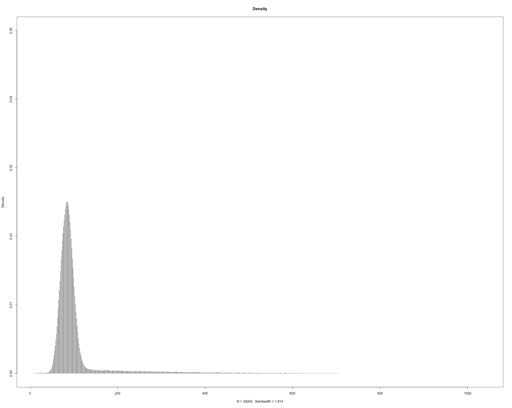
\includegraphics[width=\linewidth]{images/mema-dens-triple/I3}
    				 \end{minipage}
    			   & \begin{minipage}{.15\textwidth}\vspace{2pt}     							
     			 	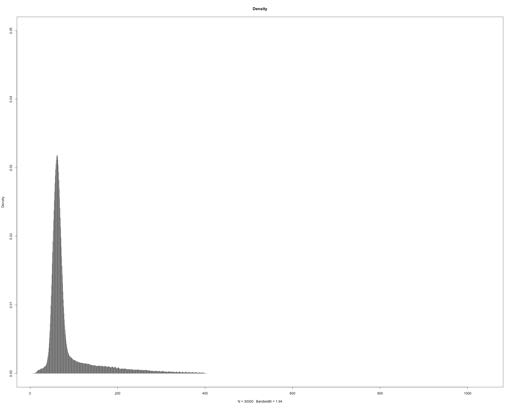
\includegraphics[width=\linewidth]{images/mema-dens-triple/I7}
    				 \end{minipage}
    			   &	 \begin{minipage}{.15\textwidth}\vspace{2pt}     							
     			 	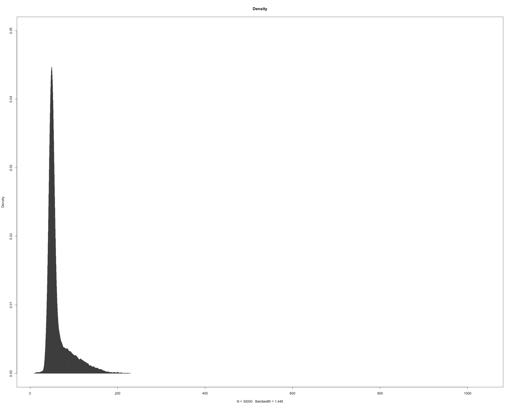
\includegraphics[width=\linewidth]{images/mema-dens-triple/I10}
    				 \end{minipage}\\	
		1000   &	 \begin{minipage}{.15\textwidth}\vspace{2pt}     							
     			 	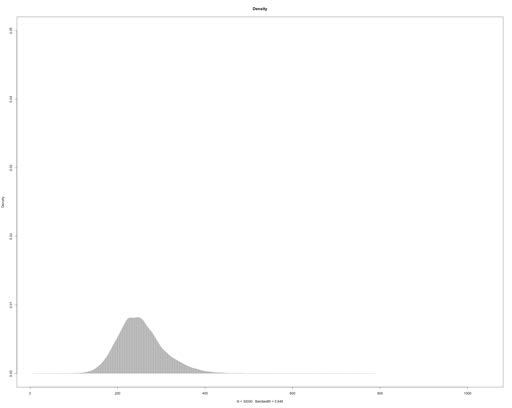
\includegraphics[width=\linewidth]{images/mema-dens-triple/I4}
    				 \end{minipage}
    			   &	 \begin{minipage}{.15\textwidth}\vspace{2pt}     							
     			 	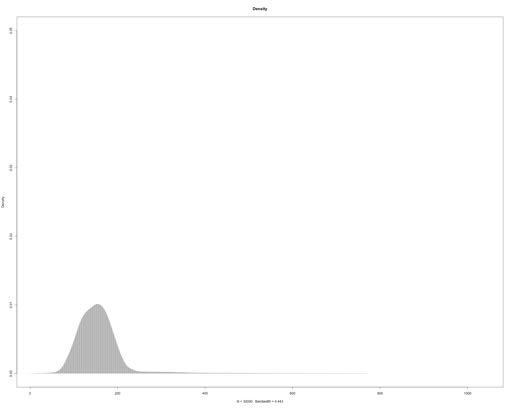
\includegraphics[width=\linewidth]{images/mema-dens-triple/I8}
    				 \end{minipage}
    			   &	 \begin{minipage}{.15\textwidth}\vspace{2pt}     							
     			 	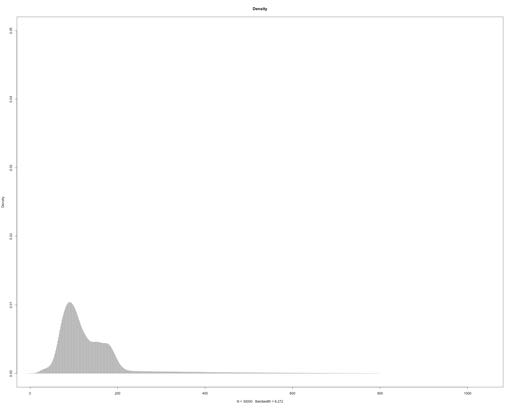
\includegraphics[width=\linewidth]{images/mema-dens-triple/I11}
    				 \end{minipage}
    			   &	 \begin{minipage}{.15\textwidth}\vspace{2pt}     							
     			 	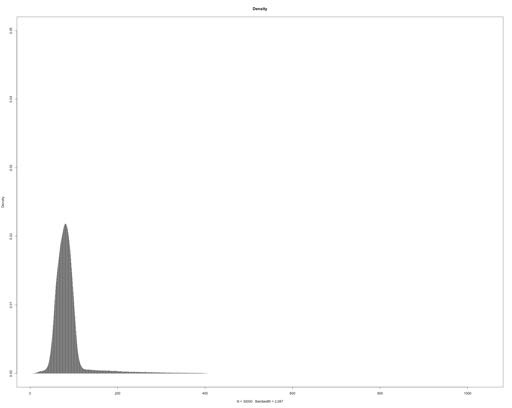
\includegraphics[width=\linewidth]{images/mema-dens-triple/I13}
    				 \end{minipage}\\
		10000  &	 \begin{minipage}{.15\textwidth}\vspace{2pt}     							
     			 	
\includegraphics[width=\linewidth]{images/mema-dens-triple/I5}
    				 \end{minipage}
    			   &	 \begin{minipage}{.15\textwidth}\vspace{2pt}     							
     			 	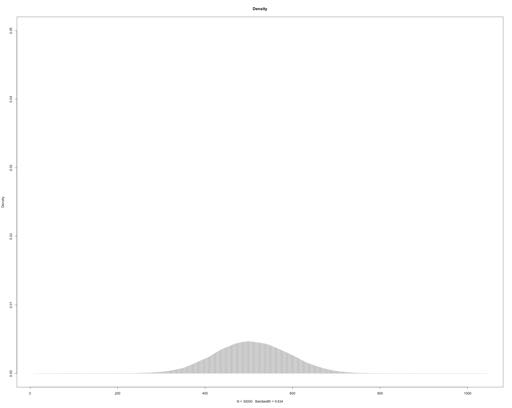
\includegraphics[width=\linewidth]{images/mema-dens-triple/I9}
    				 \end{minipage}
    			   &	 \begin{minipage}{.15\textwidth}\vspace{2pt}     							
     			 	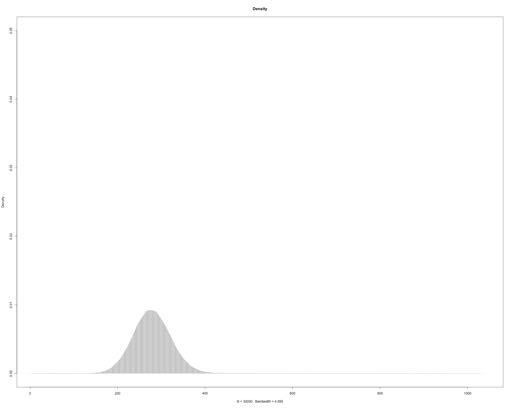
\includegraphics[width=\linewidth]{images/mema-dens-triple/I12}
    				 \end{minipage}
    			   &	 \begin{minipage}{.15\textwidth}\vspace{2pt}     							
     			 	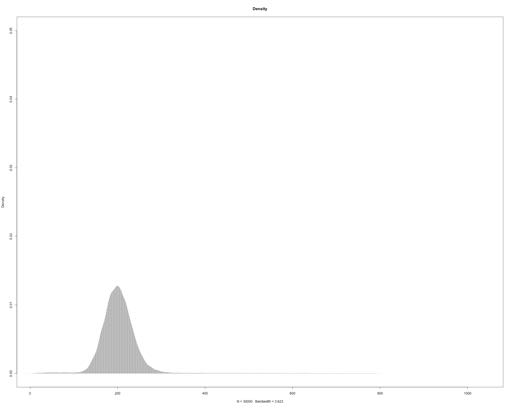
\includegraphics[width=\linewidth]{images/mema-dens-triple/I14}
    				 \end{minipage}
    			   &	 \begin{minipage}{.15\textwidth}\vspace{2pt}     							
     			 	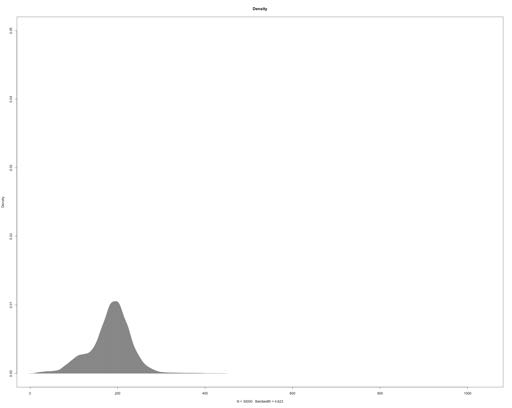
\includegraphics[width=\linewidth]{images/mema-dens-triple/I15}
    				 \end{minipage}\\
		\hline % inserts single-line
	 \end{tabular}
	}
	\caption[\textsc{Analyser} Investigation Stack - Level 2 - Pattern Identification - Memory Distribution - Baselines TN and TI]{	Figure shows how memory values for TN (a) and TI (b) are distributed over ten intervals between the global  minimum and maximum of all the SOAK tests results}�
	\label{tab:level2-memory-density-triple}
	\end{table}